\begin{figure}[h]
    \centering
    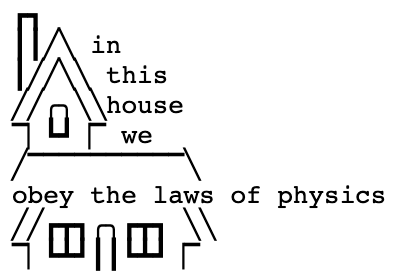
\includegraphics[height=3.5cm]{in-this-house}
\end{figure}

Mechanical buttons and switches demonstrate a phenomenon called \textit{switch bounce}.
This causes voltage to fluctuate for hundreds, often thousands, of microseconds when the contacts close or open.
When this fluctuation is in the indeterminate region between the logical low and high thresholds, it can cause the logic level to ``bounce'' back-and-forth between high and low until settling into the final, correct logic level.
This causes the digital circuitry or software to ``see'' multiple triggering events.

A traditional way to debounce is to introduce a simple low-pass filter using a resistor and a capacitor.
Other common hardware-based approaches use digital feedback circuits.
Hardware design can be simplified, and manufacturing cost can be reduced, by solving a hardware problem with software.
This, of course, transfers the design complexity to the software.

The CowPi library includes the \function{cowpi_debounce_byte()}, \function{cowpi_debounce_short()}, and \function{cowpi_debounce_long()}  functions that essentially implement a low-pass filter in software.
The functions in \textit{io\_functions.c} make use of \function{cowpi_debounce_byte()}\ifdefstring{\processor}{RP2040}{ and \function{cowpi_debounce_long()}}{}.
When you modify these functions, as long as you preserve those \function{cowpi_debounce_byte()} calls, you do not need to worry further about debouncing.
